\documentclass[conference]{IEEEtran}
\IEEEoverridecommandlockouts
% The preceding line is only needed to identify funding in the first footnote. If that is unneeded, please comment it out.
\usepackage{cite}
\usepackage{amsmath,amssymb,amsfonts}
\usepackage{algorithmic}
\usepackage{graphicx}
\usepackage{textcomp}
\usepackage{xcolor}
\usepackage{booktabs}
\usepackage{adjustbox}
\usepackage{multicol}
\usepackage{float}
\usepackage{array}

\renewcommand{\arraystretch}{1.2}

\def\BibTeX{{\rm B\kern-.05em{\sc i\kern-.025em b}\kern-.08em
    T\kern-.1667em\lower.7ex\hbox{E}\kern-.125emX}}
\begin{document}

\title{Miniproject 3 - Classification of Image Data \\
{\small COMP551 - Applied Machine Learning}
}

\author{\IEEEauthorblockN{Ege Odaci}
\IEEEauthorblockA{\textit{McGill University} \\
ege.odaci@mail.mcgill.ca}
\and
\IEEEauthorblockN{Rafael Gomes Braga}
\IEEEauthorblockA{\textit{École de Technologie Supérieure} \\
rafael.gomes-braga.1@ens.etsmtl.ca}
\and
\IEEEauthorblockN{Ramon Figueiredo Pessoa}
\IEEEauthorblockA{\textit{École de Technologie Supérieure} \\
ramon.figueiredo-pessoa.1@ens.etsmtl.ca}
}

\maketitle

\begin{abstract}
In this mini-project, we explored the task of classifying images into different labels using neural networks. We used the CIFAR-10 dataset, a collection of 60000 small color images labeled in 10 different classes, and the MNIST dataset, a collection of hand-written digits from 0 to 9. We implemented two models to perform classification, a Multilayer Perceptron and a Convolutional Neural Network. We analyzed the test and train performances of those two algorithms as a function of the epochs and compared their performance. We also studied the behavior of the Multilayer Perceptron when changing some of the parameters, such as the number of layers, number of units and type of activation. We present a detailed discussion about our results and draw some conclusions.
\end{abstract}


\section{Introduction}
\label{section:introduction}

Image classification is a process in computer science that consists of classifying images according to their content, for example, determining if it is the picture of a dog, a cat or a truck. Although this task is effortlessly performed by us humans, it is very difficult for a computer to do. In recent years artificial neural networks have been extensively used for this, mainly Convolutional Neural Networks.

In this project, we developed two neural network models to perform image classification: a Multilayer Perceptron (MLP) and a Convolutional Neural Network (CNN). We based our implementations on tutorials found online but added our modifications. For the Multilayer Perceptron, we used the matrix operations provided by the \texttt{NumPy} package and for CNN we used multiple functionalities from the \texttt{PyTorch} framework. Both models were implemented as Jupyter notebooks.

% We found out that the CNN outperforms the MLP by a large margin (30\% and 35\%, respectively). 

We trained MLP and CNN models on the CIFAR-10 dataset and compared their test accuracies. As an \textbf{extra} experiment, we also trained the MLP on the MNIST dataset to see how well it performs. Finally, we tried different configurations for the MLP, varying the number of hidden layers, number of weights and type of activation functions. We provide a discussion about the effects of varying those parameters on the accuracy.

Here is how our report is organized: Section \ref{section:related_work} gives a basic overview of the literature on artificial neural networks and image classification, Section \ref{section:datasets} describes the datasets we used and the feature extraction process, Section \ref{section:proposed_approach} describes the models we implemented, Section \ref{section:results} shows the results we obtained and Section \ref{section:discussion} provides a discussion about our findings.

\section{Related Work}
\label{section:related_work}

The Perceptron is an algorithm for supervised binary classification invented in 1958 by Frank Rosenblatt \cite{rosenblatt1957perceptron}. Although it was used for image classification since its creation, it was quickly proved that the Perceptron was not able to learn complex patterns present in images, which lead to a period of stagnation in AI research known as the AI winter\footnote{\url{https://en.wikipedia.org/wiki/Perceptron}}. Later it was found that neural networks of two or more layers (also called Multilayer Perceptrons\footnote{\url{https://en.wikipedia.org/wiki/Multilayer\_perceptron}}) trained with the backpropagation algorithm\footnote{\url{https://en.wikipedia.org/wiki/Backpropagation}} could capture more complex patterns than the single perceptron, and AI research sprang back to life in the 1980s.

Convolutional Neural Networks\footnote{\url{https://en.wikipedia.org/wiki/Convolutional\_neural\_network}} are a class of Artificial Neural Networks (ANN) that perform convolution operations over the input data and are usually applied to image classification. They were first introduced by Kunihiko Fukushima in 1980\cite{fukushima1980neocognitron}.

In the last decade, the availability of GPUs, higher processing power and large datasets made it possible to develop and train more complex Neural Network structures that achieve performances comparable or even superior to humans. In 2012 the ImageNet competition was won by Alex Krizhevsky with AlexNet \cite{krizhevsky2012imagenet}, a Deep Convolutional Neural Network (DCNN) developed at the University of Toronto. Since then, deep learning research exploded and  breakthroughs are obtained almost every year. Some examples include: VGGNet\cite{simonyan2014very}, GoogLeNet\cite{szegedy2015going} and ResNet\cite{he2016deep}.


\section{Dataset and Setup}
\label{section:datasets}

\subsection{Dataset}

The CIFAR-10 dataset is a collection of 60000 32$\times$32 color images labeled in 10 classes, 6000 images for each class. This dataset was collected by researchers at MIT and NYU over 6 months and is described in great detail in \cite{krizhevsky2009learning}. Figure \ref{fig:cifar10} shows 10 random images from each class\footnote{\url{https://www.cs.toronto.edu/~kriz/cifar.html}}.

\begin{figure}[]
\centering
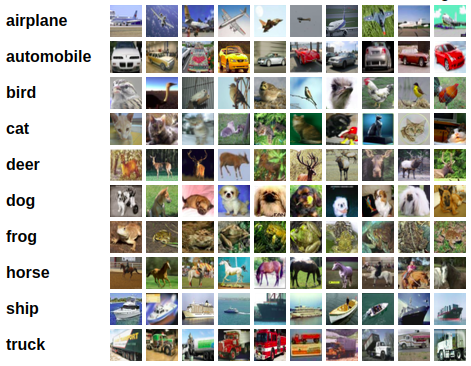
\includegraphics[scale = 0.35]{figs/cifar10.png}
\caption{Example images from each class in the CIFAR-10 dataset}
\label{fig:cifar10}
\end{figure}

There is a default test-train partition consisting of 10000 images for the test, of which there are exactly 1000 images randomly selected from each class, and 50000 images for training divided into 5 batches of 10000 images each. We used this default split in our code.

\begin{figure}[]
\centering
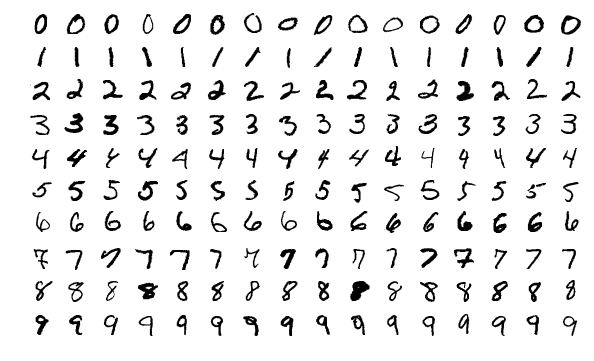
\includegraphics[scale = 0.35]{figs/mnist.png}
\caption{Example images from each class in the MNIST dataset}
\label{fig:mnist}
\end{figure}

The MNIST dataset is a collection of images of handwritten digits, created from samples of the original NIST dataset. It has 60000 images for training and 10000 for the test. Each image is a 28$\times$28 grayscale picture of a digit from 0 to 9. Since its introduction\cite{lecun1998gradient} it has been used extensively in the machine learning community. Figure \ref{fig:mnist} shows some examples of images from this dataset\footnote{\url{https://en.wikipedia.org/wiki/MNIST\_database}}.

\subsection{Feature Extraction}

Images in the CIFAR-10 dataset are 32$\times$32 pixels and they are also colored having RGB (Red, Green, Blue) values for each pixel. To represent that, we need a 32$\times$32$\times$3 multidimensional array. Similarly, the images in the MNIST dataset are 28$\times$28 grayscale pixels, represented by 28$\times$28$\times$1 matrices. To be able to feed this data to our networks, we first flattened the samples, turning them into column vectors. For the CIFAR-10 dataset this means 3072 dimensions vectors and for MNIST, 784 dimensions vectors. 

\section{Proposed Approach}
\label{section:proposed_approach}

\subsection{Multilayer Perceptron}

The Multilayer Perceptron is a more complex version of the Perceptron algorithm, in which layers of units, or neurons (each one performing the Perceptron algorithm) are stacked. Data is fed to the \textbf{input layer}, which processes it and sends it forward to the various \textbf{hidden layers}. After the data passes through all the hidden layers it gets to the \textbf{output layer}, which contains exactly one neuron for each class, that is going to output a score representing how likely that data is from belonging to that specific class. We then select the class with the highest output as our classification decision. Figure \ref{fig:mlp} shows the structure of a typical network like this\footnote{\url{http://www.texample.net/tikz/examples/neural-network/}}.

\begin{figure}[]
\centering
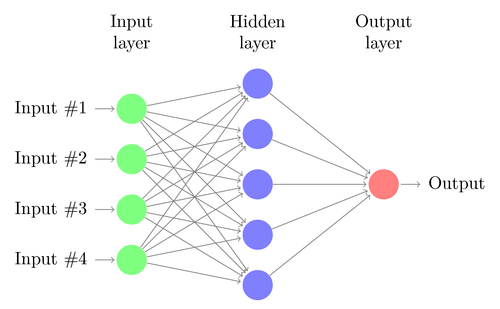
\includegraphics[scale = 0.45]{figs/mlp.png}
\caption{Structure of a typical Multilayer Perceptron}
\label{fig:mlp}
\end{figure}

In the simplest form of network each neuron is fully connected with all neurons in the previous layer - we call that a \textbf{dense layer}. In this case, each neuron is performing a linear combination of the data that is coming from the previous layer, multiplying each value for weight and then adding a bias. Then, a nonlinear activation function is applied and the result is sent to the next layer. There are many possible options for this activation function and we tested some of the more popular ones.

To train the network we first calculate the error between the network's prediction about a specific sample and the actual label of that sample. We then calculate the gradient that needs to be applied to the weights to minimize that error and propagate this error back through the network using the chain rule for partial derivatives. This famous algorithm is called the backpropagation algorithm. After this is done for a sufficient number of samples the network learns to recognize patterns in the input data and classify it into the possible classes.

We based our implementation on this tutorial\cite{mlpFromScratchTutorial}. The dense layers are implemented as Python classes and the activation functions are also implemented as classes that can perform both the forward and backward passes in a layer considering the specific activation function that is being used. To try different configurations for our network, we implemented four types of activation functions: ReLU, Leaky ReLU, TanH and, Sigmoid.

The network can be built by stacking the desired layers in a list structure. The number of layers and the number of neurons in each layer can be chosen when building this structure. We tried different architectures and report our findings in the Section \ref{section:results}.

To train the network we call the forward and backward functions from each layer. The training loop is implemented as a Stochastic Gradient Descent (SGD) algorithm to speed up the training process. In this algorithm instead of using all the data for training, we only process a small portion of it each time, called a mini-batch. The algorithm can be stopped when the desired accuracy is obtained, without the need to go through all the data. Again, to experiment with the code, we tested different mini-batch sizes.

The code is implemented as a Jupyter notebook and all main steps and decisions are documented in text cells and comments in the code.

\subsection{Convolutional Neural Network}

The Convolutional Neural Network (CNN) is one example of a deep learning algorithm. It is a huge step forward in the image recognition task. They are very useful when we need to analyze an image in image classification\cite{CNNnetwork}. CNN is widely used, from photo tagging to self-driving cars. The architecture behind CNN is similar to how neurons in our brain act\cite{CNNnetwork}.

\begin{figure}[H]
\centering
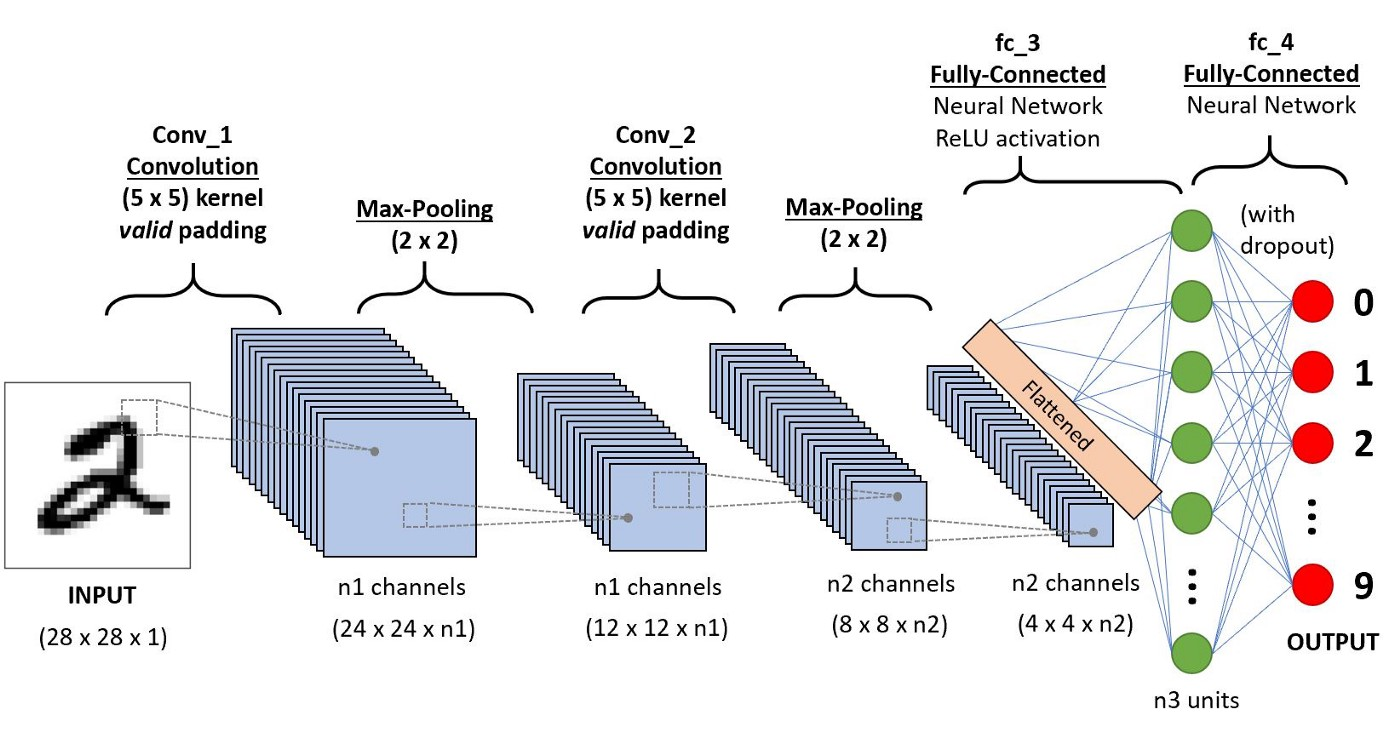
\includegraphics[scale = 0.18]{figs/CNN.jpeg}
\caption{Structure of a convolutional neural Network}
\label{fig:CNNstructire}
\end{figure}

The input image is processed through convolutional layers applying convolution operation and passing the input to the next layers as can be seen in Figure \ref{fig:CNNstructire} \footnote{\url{https://miro.medium.com/max/1400/1*uAeANQIOQPqWZnnuH-VEyw.jpeg}}. Then the pooling layer is applied and finally, the vector is passed into a fully connected neural network\cite{CNNnetwork}.

\section{Results}
\label{section:results}

We ran our implementation of MLP on the given dataset CIFAR-10, obtaining training and test accuracy of 10\% as can be seen in Figure \ref{fig:Cifar10Train}. We tried debugging it and found out that an overflow happens in the softmax function. After some iterations the weights grow too large resulting in infinity, causing the overflow. We have tried several approaches to solve this issue but unfortunately, none worked on time. Our final code is in the file \texttt{group10\_1-MLP-CIFAR10.ipynb}.

\begin{figure}[H]
\centering
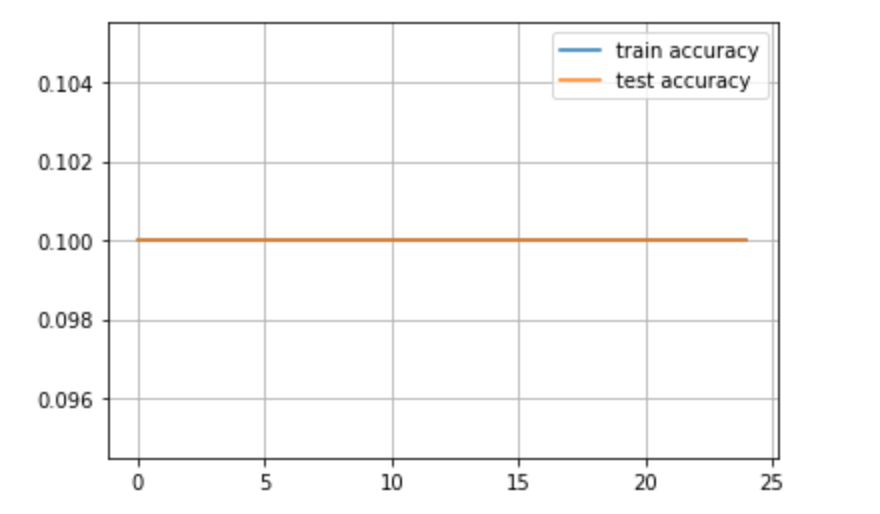
\includegraphics[scale = 0.50]{figs/trainandtestMLP.png}
\caption{Training and test accuracy per epoch for the MLP algorithm in the Cifar-10 dataset }
\label{fig:Cifar10Train}
\end{figure}

On the other hand, we have tested our implementation of MLP using a different dataset called MNIST. This version is in the file \texttt{group10\_2-MLP-MNIST.ipynb}. We have obtained better results for this dataset as can be seen in the next parts of the report.
We have tested 4 different dense layers (2 to 5), 4 different learning rates, 5 different batch sizes, and 4 different activation functions.

\begin{figure}[H]
\centering
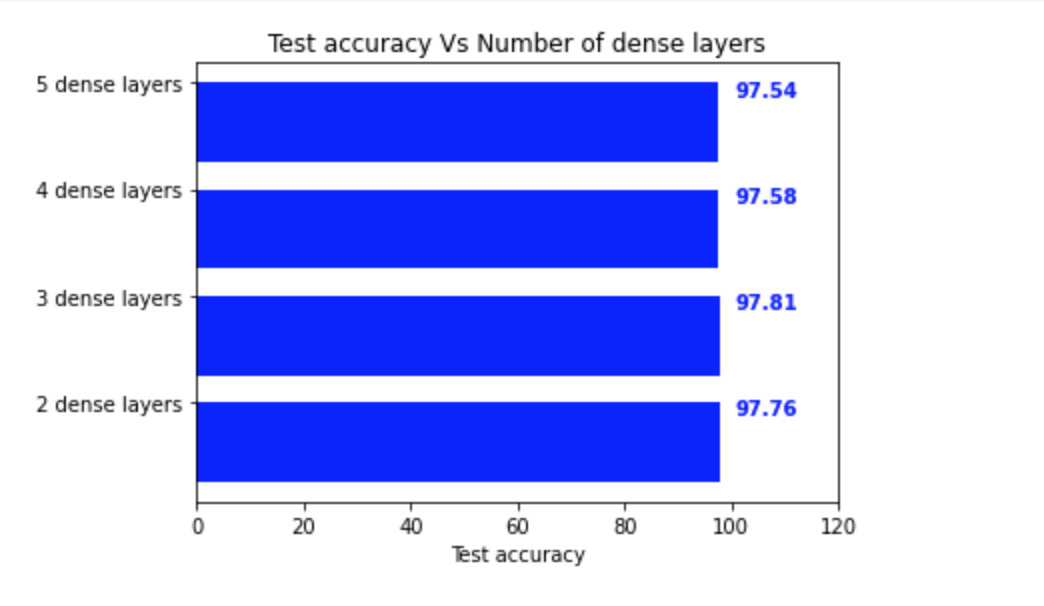
\includegraphics[scale = 0.50]{figs/layers_MNIST.png}
\caption{Number of layers vs test accuracy for MNIST}
\label{fig:layersMNIST}
\end{figure}

\begin{figure}[H]
\centering
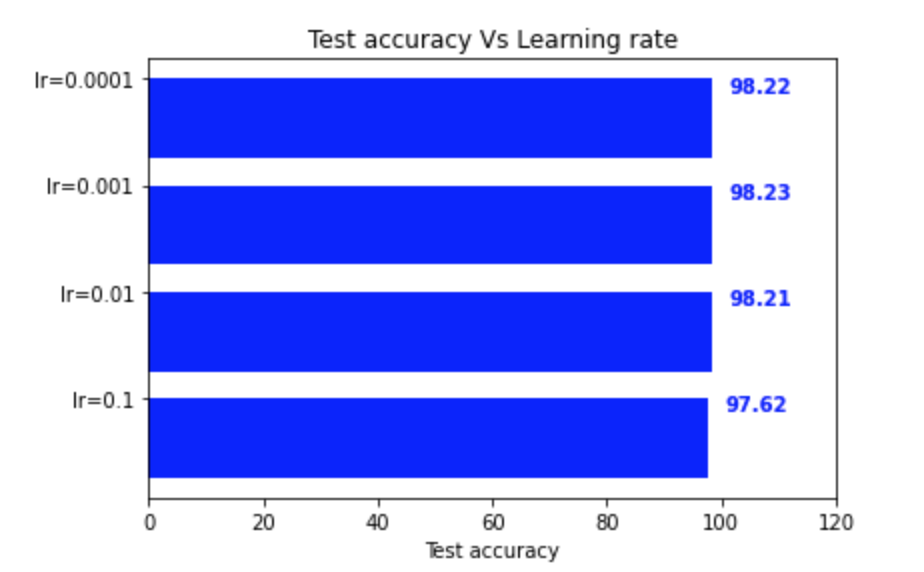
\includegraphics[scale = 0.50]{figs/learningrate_MNIST.png}
\caption{Learning rate vs test accuracy for MNIST}
\label{fig:learningRateFunctionMNIST}
\end{figure}

\begin{figure}[H]
\centering
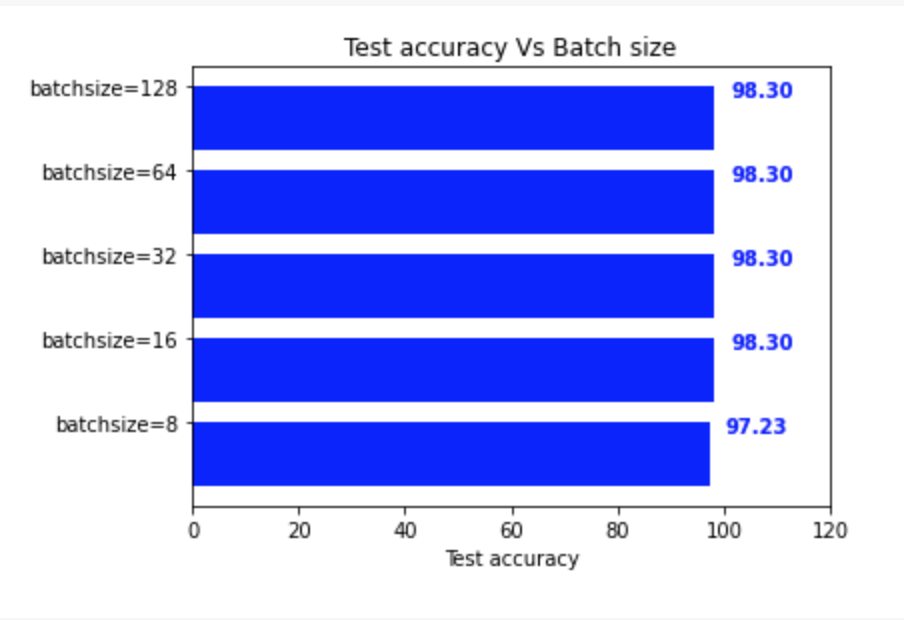
\includegraphics[scale = 0.50]{figs/batchsize_MNIST.png}
\caption{Batch size vs test accuracy for MNIST}
\label{fig:batchsizeMNIST}
\end{figure}

\begin{figure}[H]
\centering
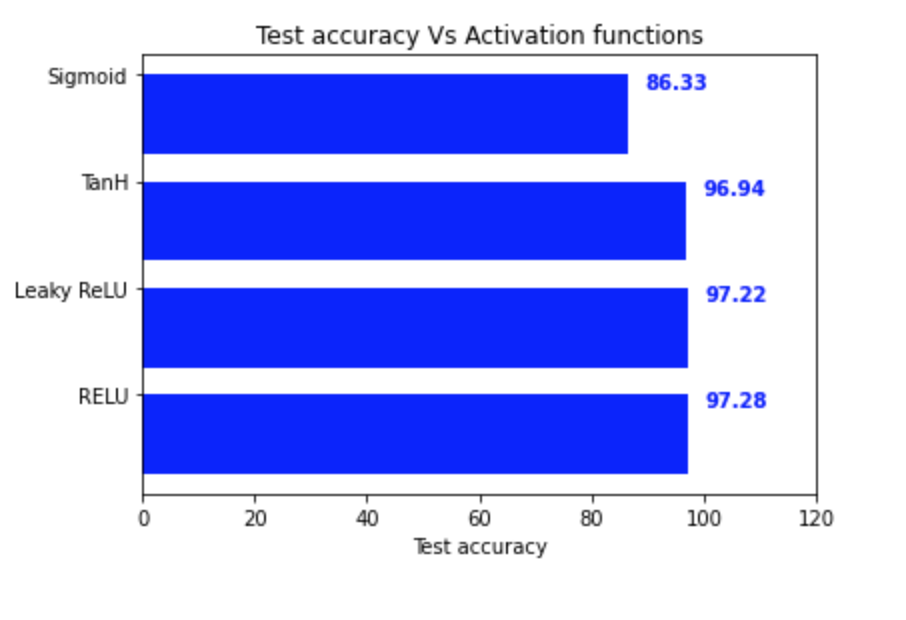
\includegraphics[scale = 0.50]{figs/activationFunctions_MNIST.png}
\caption{Activation functions vs test accuracy for MNIST}
\label{fig:activationFunctionsMNIST}
\end{figure}

To find the optimal number of dense layers, we tested different numbers as can be seen in Figure \ref{fig:layersMNIST}. We found that use 3 dense layers give the best result. We tested different learning rates for our model and concluded that 0.001 works better (see Figure \ref{fig:learningRateFunctionMNIST}). Our algorithm was tested using batch sizes of 8, 16, 32, 64, and 128 and we found no improvement increasing the batch size after 16 as can be seen in Figure \ref{fig:batchsizeMNIST}. Finally, we have tested different activation functions for our algorithm, results in Figure \ref{fig:activationFunctionsMNIST}, and found out that the RELU activation function gives us the highest result. Combining all these results we have picked the best parameters as follows: Using 3 dense layers with learning rate=0.001, activation function as RELU and mini-batches with a batch size of 32. 

\begin{figure}[H]
\centering
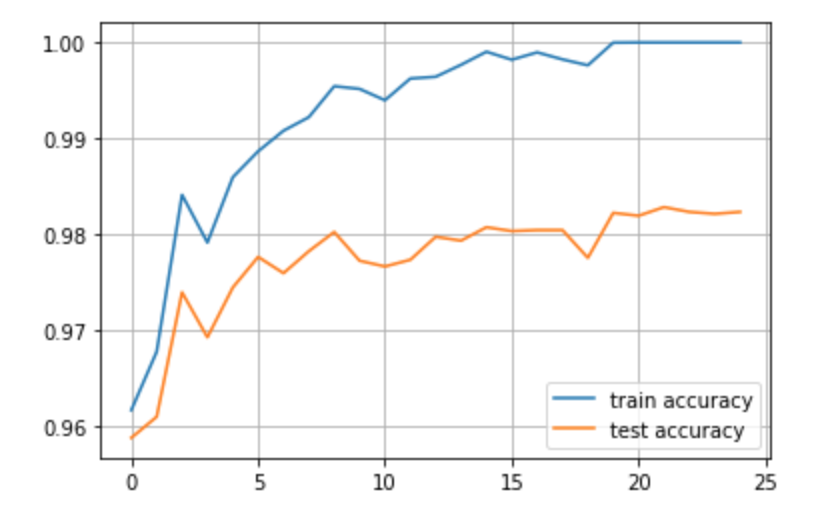
\includegraphics[scale = 0.50]{figs/newtrainandtestMNIST.png}
\caption{Training and test accuracy per epochs for the MLP algorithm in the MNIST dataset with best parameters}
\label{fig:bestTrainingandTestAccMNIST}
\end{figure}

\begin{figure}[H]
\centering
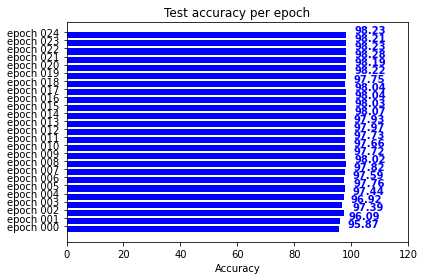
\includegraphics[scale = 0.50]{figs/bestTestAcc_MNIST.png}
\caption{Test accuracy per epochs for the MLP algorithm in the MNIST dataset with best parameters}
\label{fig:bestTestAcc_MNIST}
\end{figure}

\begin{figure}[H]
\centering
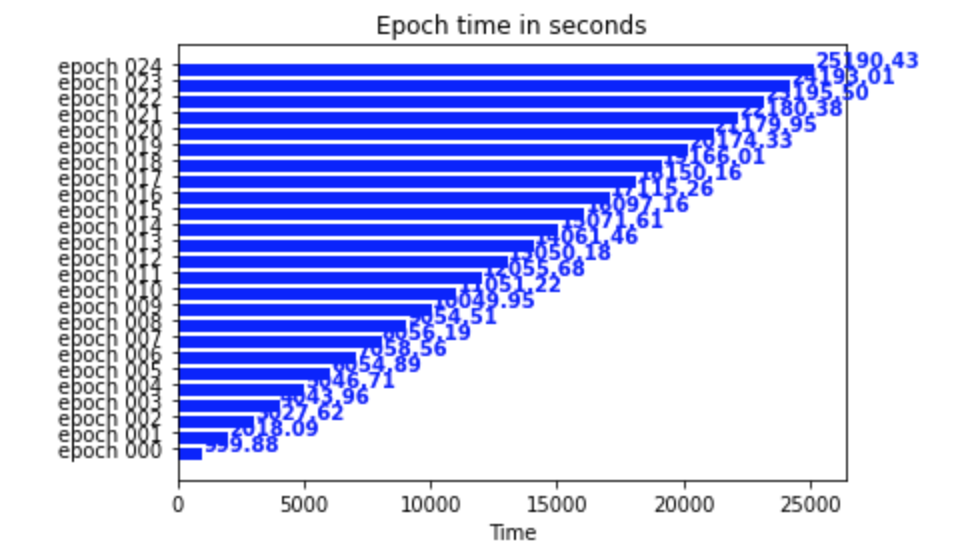
\includegraphics[scale = 0.50]{figs/bestParamsEpocTimes_MNIST.png}
\caption{Runtime per epochs for the MLP algorithm in the MNIST dataset with best parameters}
\label{fig:bestRuntimeEpochMNIST}
\end{figure}

When we run the algorithm with the best parameters we can see that our train accuracy reaches 100\% after the 18th epoch and our test accuracy reaches 98.23\% after the 23rd epoch (see Figure \ref{fig:bestTrainingandTestAccMNIST} and \ref{fig:bestTestAcc_MNIST}) for the MNIST dataset. We also see a linear increase in runtimes as our program does more epochs as can be seen in Figure \ref{fig:bestRuntimeEpochMNIST}.

\medskip

\begin{table}[H]
\caption{CNN PyTorch tutorial: accuracy for each class of CIFAR10 dataset}
\label{table:cifar10CNN}
\begin{center}
\begin{adjustbox}{max width=0.99\textwidth}
\begin{tabular}{|l|l|}
\hline
   Experiment                   & Accuracy(\%)   \\
  \hline
 Plane           & 76\%                 \\
 Car           & 79\%                 \\
 Bird           & 33\%                 \\
 Cat           & 35\%                 \\
 Deer           & 47\%                 \\
 Dog           & 45\%                 \\
 Frog           & 72\%                 \\
 Horse           & 58\%                 \\
 Ship           & 45\%                 \\
 Truck           & 55\%                 \\
\hline
\end{tabular}
\end{adjustbox}
\end{center}
\end{table}

For CNN using PyTorch, we have followed the tutorial given by COMP 551's assignment 3 and we include detailed comments for the tutorial code. The Jupyter notebook with comments can be found in a notebook called \texttt{group10\_Tutorial\_CIFAR10\_CNN\_PyTorch.ipynb}. Table \ref{table:cifar10CNN} shows CNN accuracy for each class of CIFAR10 dataset. The accuracy of the network on the 10000 test images using the tutorial code with 2 epochs is 55\%.

Table \ref{table:summaryAlgorithm} summarizes the best accuracy we obtained for each model and dataset we tried. The Jupyter notebook with Keras implementation of MLP and CNNs can be found in a notebook called \texttt{group10\_3-CIFAR10\_Keras.ipynb}: Keras MLP classifier, Keras CNN classifier, Keras regularization using dropout and batch normalization, and data augmentation with Keras.

\begin{table}[H]
\caption{Compare test accuracy on different datasets for various algorithms}
\label{table:summaryAlgorithm}
\begin{center}
\begin{adjustbox}{max width=0.99\textwidth}
\begin{tabular}{|l|l|l|}
\hline
   Dataset       & Algorithm         & Accuracy (\%)   \\
  \hline
 CIFAR10      & MLP: 3 dense layers, RELU, batchsize = 32 &   10.00 \%                 \\
   \hline

 MNIST       & MLP: 3 dense layers, RELU, batchsize = 32 &   98.23 \%                 \\
   \hline

  CIFAR10      & PyTorch: CNN (Tutorial), epochs = 2     &   55.00 \%                 \\
    \hline

   CIFAR10      & Keras: MLP, epochs = 15 &   48.21 \%                 \\
     \hline

    CIFAR10      & Keras: CNN, epochs = 15 &    64.09\%                 \\
      \hline

     CIFAR10      & Keras: CNN dropout, batch norm., ep=15 &   71.35 \%      
     \\
       \hline

 CIFAR10      & Keras: CNN with data augmentation, ep=15     &   68.58 \%                 \\
   \hline

\hline
\end{tabular}
\end{adjustbox}
\end{center}
\end{table}

\section{Discussion and Conclusion}
\label{section:discussion}

We were able to obtain pretty good results for the MLP model in the MNIST dataset, however, we ran into an issue with the CIFAR-10 dataset, which contains color, and more complex images. For this dataset the network weights grow too large very fast, causing an overflow when calculating the cross-entropy loss. The result is that the network fails to predict the correct label for the images, obtaining 10\% accuracy. We tried many strategies to fix this issue, such as adding regularization, scaling the exponential function in the cross-entropy loss, but none of them worked and we ran out of time.

Since we couldn't fix that issue, we focused our efforts on the MNIST dataset and performed many different tests by varying the number of layers, activation functions, learning rate and mini-batch sizes of the stochastic gradient descent algorithm. Since the accuracy of this dataset was already very good with just the initial parameters, we didn't see much change in the results for each of those experiments. The biggest change we observed was the use of the Sigmoid function as activation, which obtained a significantly lower accuracy than the other functions.

The CNN, however, obtains an acceptable accuracy on the CIFAR-10 dataset, which shows how well this type of model works with image classification tasks, compared to the basic MLP. This is due to the network's more complex architecture, which was developed specifically for this type of task.

In conclusion, we learned that CNNs are a lot more suited to work with complex, colored images than simple MPLs. For future works we would like to solve the overflow problem we encountered in our MLP implementation and then trying new strategies to improve its accuracy, for example, using transfer learning and ensemble methods. We also think it would be interesting to try new CNN configurations as we did for the MLP.

\section{Statement of Contributions}
\label{section:contributions}

Ege included comments in the tutorial of CNN using PyTorch (Jupyter notebook) and worked on the results section of the report. He also helped to fix some issues in the code. Rafael implemented the activation functions and wrote the introductory sections and the proposed approach section of this report. Ramon developed the Jupyter notebooks, implemented the MLP algorithm and supporting functions, developed the tests with different configurations, and worked in the report.

\medskip

\small

\bibliography{bibliography}


\bibliographystyle{ieeetr}

\end{document}
